%%%%%%%%%%%%%%%%%%%%%%%%%%%%%%%%%%%%%%%%%%%%%%%%%%%%%%%%%%%%

%
% "Evoflock: evolved inverse design of multi-agent motion"
% speculative draft paper
%
% May 29, 2025  Begin draft.
%
%%%%%%%%%%%%%%%%%%%%%%%%%%%%%%%%%%%%%%%%%%%%%%%%%%%%%%%%%%%%

\documentclass[letterpaper]{article}
\usepackage{natbib,alifeconf}

% Used for ALife, not sure I still need them.
\usepackage{calc}
\usepackage[hyphens]{xurl}
\usepackage{hyperref}
\usepackage{tabularx}

% Added 20230421 to allow SIGGRAPH-style “teaser figure'' under title.
\usepackage{authblk}
\usepackage{titlepic}
\usepackage{caption}
\usepackage{float}
\usepackage[T1]{fontenc} % ??? QQQ -- "<"

%%%%%%%%%%%%%%%%%%%%%%%%%%%%%%%%%%%%%%%%%%%%%%%%%%%%%%%%%%%%

% \graphicspath{ {images/} {images/fcd5/} }
\graphicspath{ {images/} }

%% For introducing terms which have a special meaning in this work.
\newcommand{\jargon}[1]{\textit{#1}}

%% Use like: {\runID backyard\_oak\_20230113\_2254}
\newcommand{\runID}{\footnotesize}

%% for laying out a row of 4, 6, or 9 images
\newcommand{\igfour}[1]{\includegraphics[width=0.24\linewidth]{#1}}
\newcommand{\igsix}[1]{\includegraphics[width=0.16\linewidth]{#1}}
\newcommand{\ignine}[1]{\includegraphics[width=0.104\linewidth]{#1}}

% small fixed-width font
\newcommand{\stt}[1]{{\small \texttt{#1}}}

%%%%%%%%%%%%%%%%%%%%%%%%%%%%%%%%%%%%%%%%%%%%%%%%%%%%%%%%%%%%

\begin{document}

\title{Evoflock: evolved inverse design of multi-agent motion}

\author{Craig Reynolds\authorcr
    unaffiliated researcher\authorcr 
    cwr@red3d.com}

%%%%%%%%%%%%%%%%%%%%%%%%%%%%%%%%%%%%%%%%%%%%%%%%%%%%%%%%%%%%

\captionsetup{hypcap=false}

\titlepic{
\includegraphics[width=\textwidth]{images/temp_fig_1.png}
\captionof{figure}{800 boids flocking in a space cluttered with obstacles. Behavioral parameters of the boids are determined by inverse design, using multi-objective evolutionary optimization.} 
\label{fig:boid_flock}}

% Remove today's date being inserted after the title/author information.
\date{}

%% Lay out the single column top matter defined above.
\maketitle

% This puts a page number at the bottom center, but too close to text.
% \pagestyle{plain}
% \pagenumbering{arabic}

%%%%%%%%%%%%%%%%%%%%%%%%%%%%%%%%%%%%%%%%%%%%%%%%%%%%%%%%%%%%

\begin{abstract}
    This paper describes an automatic method for \textit{adjusting} or \textit{tuning} models of multi-agent motion. Simulating the motion of bird flocks, human crowds, vehicle traffic, and other multi-agent systems is a widely used technique. These simulations model the behavior of a single group member (bird, human, or vehicle). The group behaviors (flock, crowd, traffic) \textit{emerge} from interactions between group members. These models usually have many numeric control parameters. Although each parameter may be intuitive in isolation, their interaction can be complex and nonlinear. It can be difficult to know how to adjust which parameters to make a desired change in the group behavior. Changing one aspect of group behavior often causes other aspects to change, leading to a long frustrating process of incremental changes. In this work, the desired group behavior is measured with an objective(/fitness/loss) function and optimized with a \textit{genetic algorithm}.

    [[[\textbf{...maybe explicitly mention the components of my objective function?...}]]]

    [[[\textbf{...maybe an ``Interestingly...'' mention of how alignment just emerges out of learning to maintain a given interval of separation...}]]]
\end{abstract}

\noindent{\small\textbf{Keywords:} boids, inverse design, optimization, evolutionary computation, genetic algorithm, flocks, herds, schools, crowds, traffic}

%%%%%%%%%%%%%%%%%%%%%%%%%%%%%%%%%%%%%%%%%%%%%%%%%%%%%%%%%%%%

\begin{figure*}[t]
    \centering
    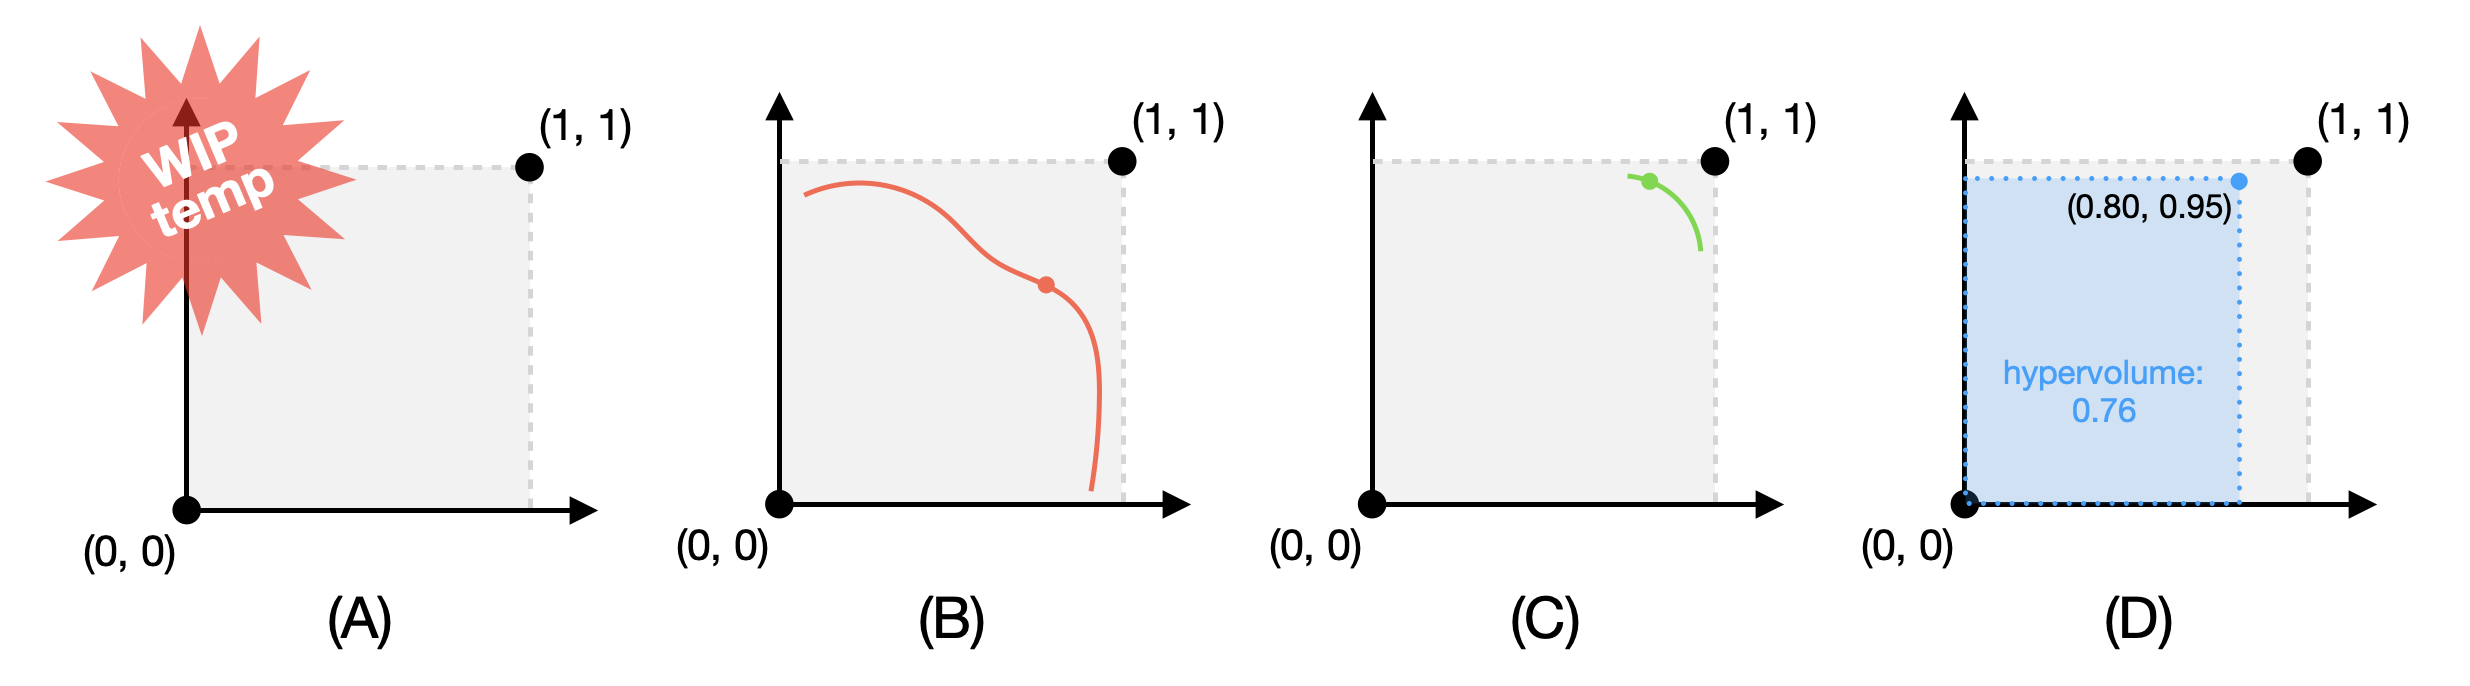
\includegraphics[width=0.9\textwidth]{images/temp_MOF_HV.png}
    \caption{(A) Normalized multi-objective fitness space. For two objectives, a unit square. (B) The \textit{Pareto front} for two mutually conflicting objectives. (Like \textit{reliability} and \textit{affordability} in the hypothetical bridge design example.) The objectives can not all be fully satisfied at any point along the front. Visually, this is the ``distance'' from (1, 1) to the red curve. (C) Two ``mostly compatible'' objectives, more typical of criteria for flock tuning. Here, the Pareto front passes near the global optimum. (D) Scalarization of a multiple-objective fitness value, using \textit{hypervolume}: the product of all objective scores. In this 2D example it is the blue rectangle's \textit{area}. Solving a multi-objective problem using scalarized fitness works best for problems of type (C).}
    \label{fig:MOF_HV}
\end{figure*}

%%%%%%%%%%%%%%%%%%%%%%%%%%%%%%%%%%%%%%%%%%%%%%%%%%%%%%%%%%%%

\section{Introduction}
\label{sec:intro}

Simulation models of multi-agent motion are used in many fields. These include animation, games, biology, robotic swarms, urban planning, and training autonomous vehicles. Since the 1980s, several models of group motion have been developed, including \textit{boids} and others. See \nameref{sec:related}. These allow creating simulations of flocks and other group motions, which most observers recognize as some type of flocking. This paper will refer to bird flocks, with the assumption that other types of group motion (herds, schools, crowds, traffic, drone swarms) can also be portrayed.

This project addresses the issue of \textit{adjusting} or \textit{tuning} multi-agent motion models, toward a given behavioral goal. For example, modifying a model of bird flocks to instead portray fish schools. Or start from a model of flocking crows and change it to represent flocking sparrows. Or to take a plausibly realistic model of a natural bird flock, and change it, say for storytelling purposes, to convey a flock of birds that are happy, or angry. Similarly, starting from a generic abstract flock model and fitting it to field observations of a given species of real birds in nature.

A boids-like simulation model typically has a collection of numeric parameters (``knobs'') that control its action. The theme of this work is a software framework that automatically finds a set of near-optimal parameters for a simulation-based multi-agent system. The flock model used for these experiments is a predefined hand-written ``black box'' model whose input is a \textit{parameter set} (consisting of about [[[\textbf{15}]]] numbers, see Table \ref{table:flock-parameters}). The user provides a \textit{fitness} (also known as \textit{objective} or \textit{loss}) function. It takes a candidate parameter set, runs a simulation, and returns a score reflecting how well the behavioral goals were met. The optimization process runs (for about two hours on a laptop) and produces a high quality parameter set, as measured by the objective function.

For a user of this optimization framework, it is convenient that the flock model is treated as a black box. Almost no restrictions are imposed on a preexisting model by the optimization framework. There are no restrictions on model design, its mutability, or the programming language used. (The latter can be an issue if optimization requires language tools such as automatic differentiation \citep{baydin_automatic_2018}.)

In the past, flock models have been tuned manually. That can be a frustrating and time-consuming process. For a new model, adjusting parameters is required simply to create group motion that looks like plausible flocking. Any modification to a group motion model (e.g. birds{$\rightarrow$}fish) requires further adjustments to the parameters. Each such adjustment requires selecting which parameter(s) to change, whether it should increase or decrease, and by how much. Often more than one parameter needs to be changed. The main difficulty is that effects of control parameters may overlap and interact in non-linear ways. Changing one usually requires changing others to compensate. Often, the result is that many parameters need to be changed, leading to a long series of changes and testing.

This paper is about automating that adjustment process using metrics of flock quality and an optimization process. The metrics use multiple objectives. The nature of those objectives and how to add new ones will be described in sections \nameref{sec:FlockingObjective} and \nameref{subsec:add_objective}. The optimization process used in these experiments is a genetic algorithm, described in section \nameref{subsec:Optimization_with_GA}.

A summary of (``hyper'')parameters for this framework is given in Table \ref{table:HyperParameters}. See \href{https://anonymous.4open.science/r/evoflock-9B09/}{anonymized c++ code} for this project. See this \href{https://drive.google.com/file/d/1ZbanvWVfapnH2TpTqamypWFoXuMeoY9b/view?usp=sharing}{video} of flock simulations based on this approach.

%%%%%%%%%%%%%%%%%%%%%%%%%%%%%%%%%%%%%%%%%%%%%%%%%%%%%%%%%%%%

\begin{figure*}[t]
    \centering
    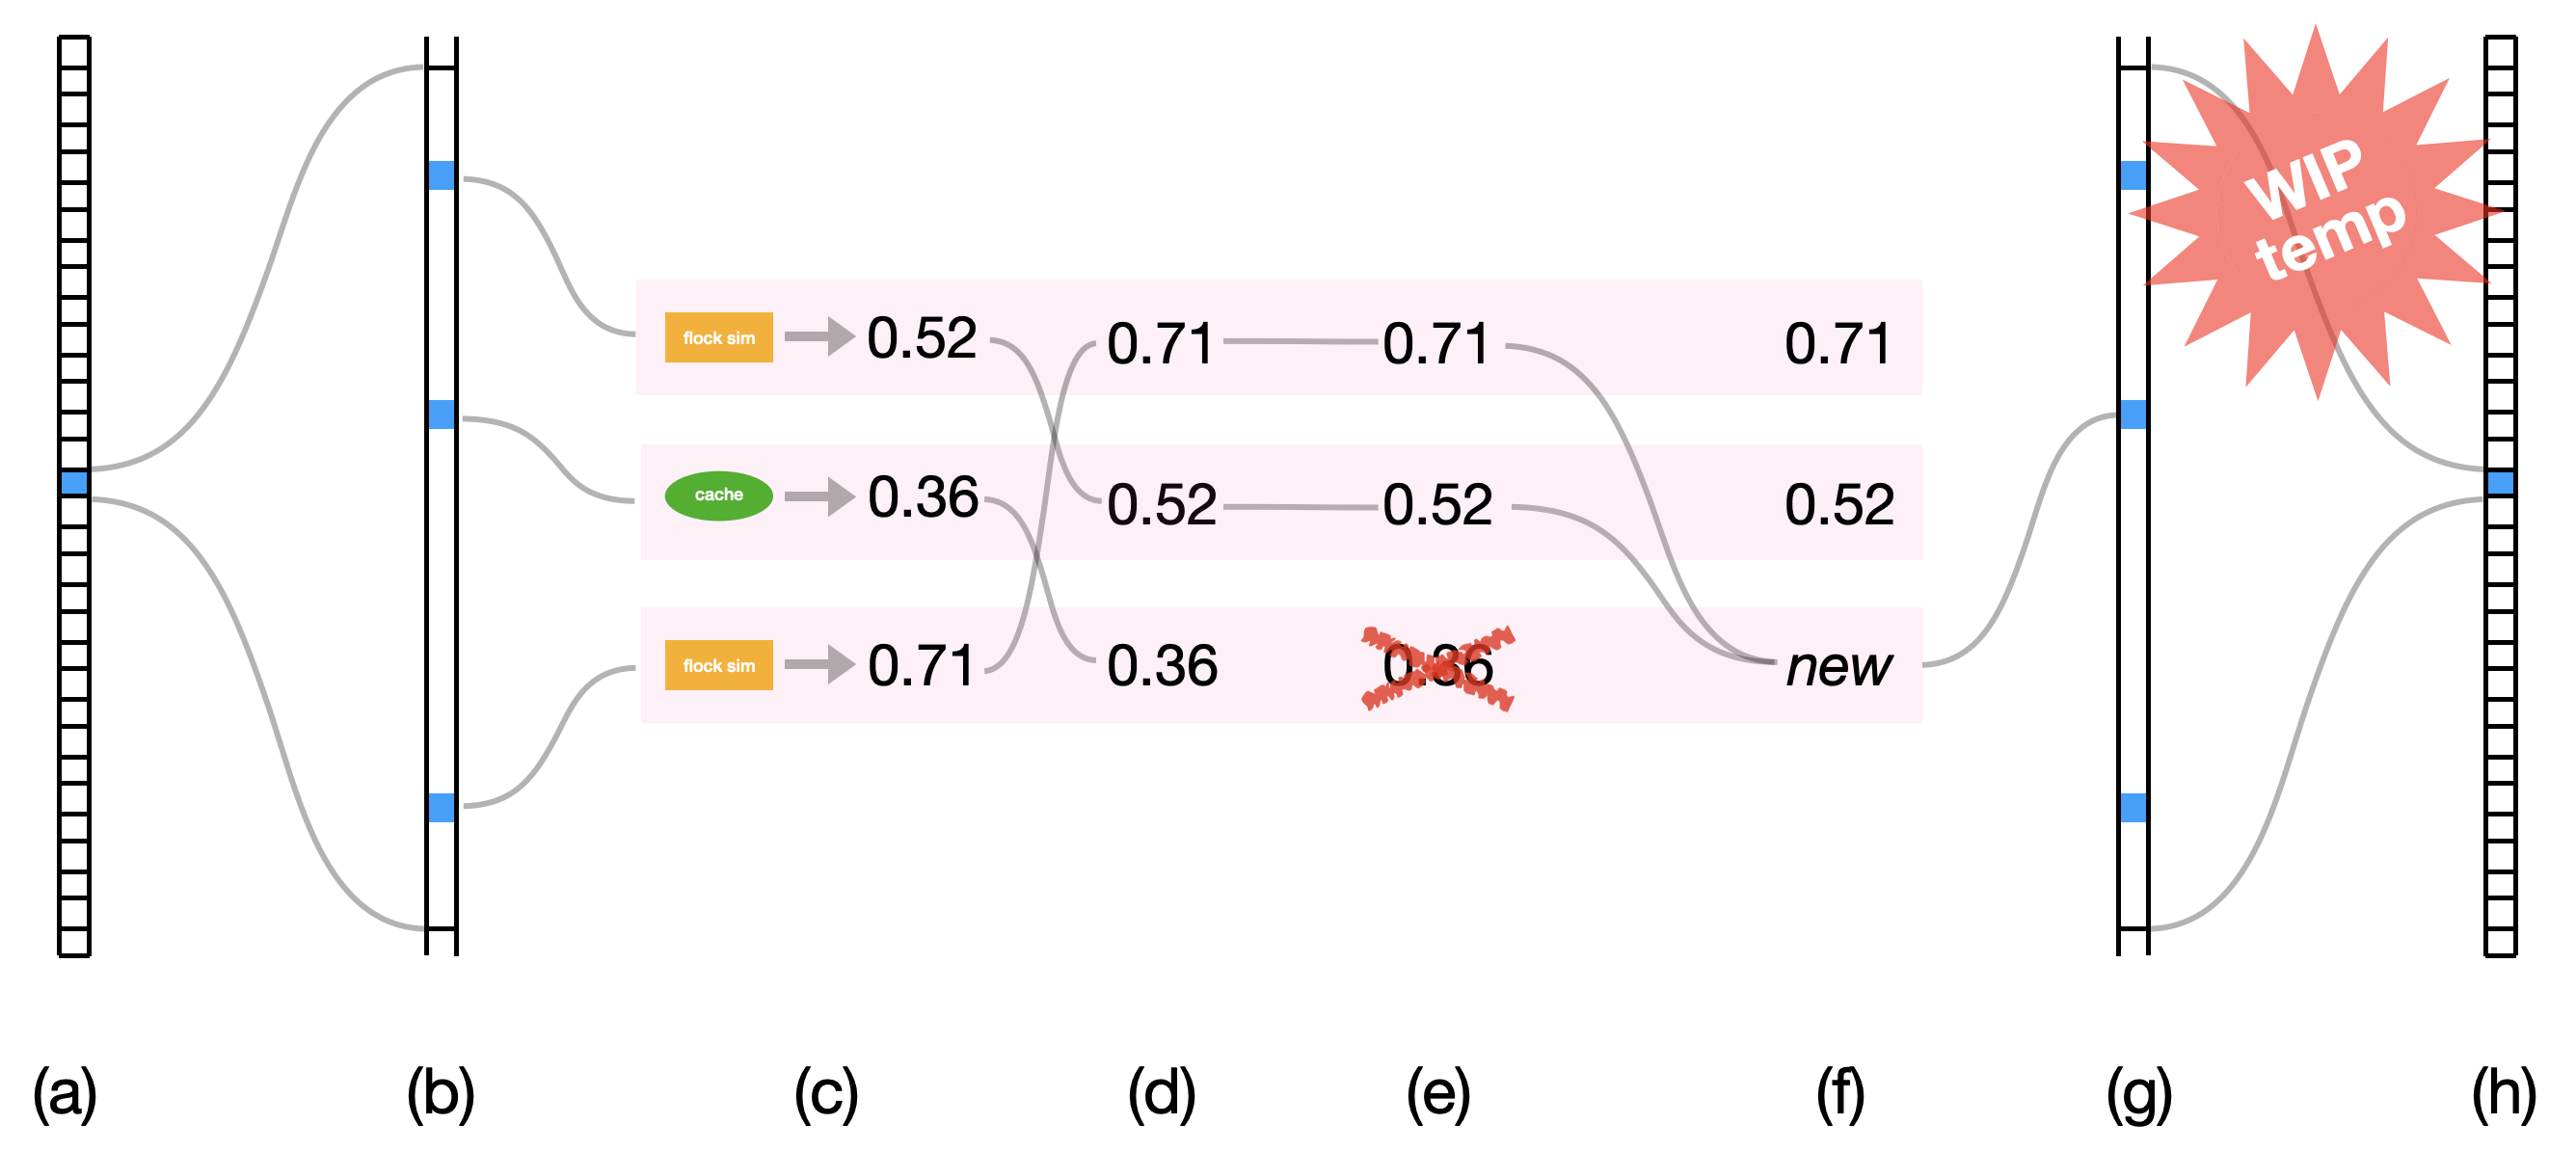
\includegraphics[width=0.7\textwidth]{images/temp_evo_update.png}
    \caption{One update step of the (SSGA) evolutionary optimization process, using a 3-way tournament: (a) uniformly select one of the \textit{sub-populations}, (b) from that sub-population, uniformly select three \textit{individuals}, each holding a flock parameter set, (c) get fitness for each, either by running flock simulations (green), or using the fitness cached from previous tournaments (orange), (d) sort the three by fitness, (e) the worst (least fit) individual is deleted, (f) the best two individuals mate (\textit{crossover}) to create a new individual, (g,h) that new individual replaces the worst of the three back in the population.}
    \label{fig:temp_evo_update}
\end{figure*}

%%%%%%%%%%%%%%%%%%%%%%%%%%%%%%%%%%%%%%%%%%%%%%%%%%%%%%%%%%%%

%%%%%%%%%%%%%%%%%%%%%%%%%%%%%%%%%%%%%%%%%%%%%%%%%%%%%%%%%%%%

\begin{figure}[t]
    \centering
    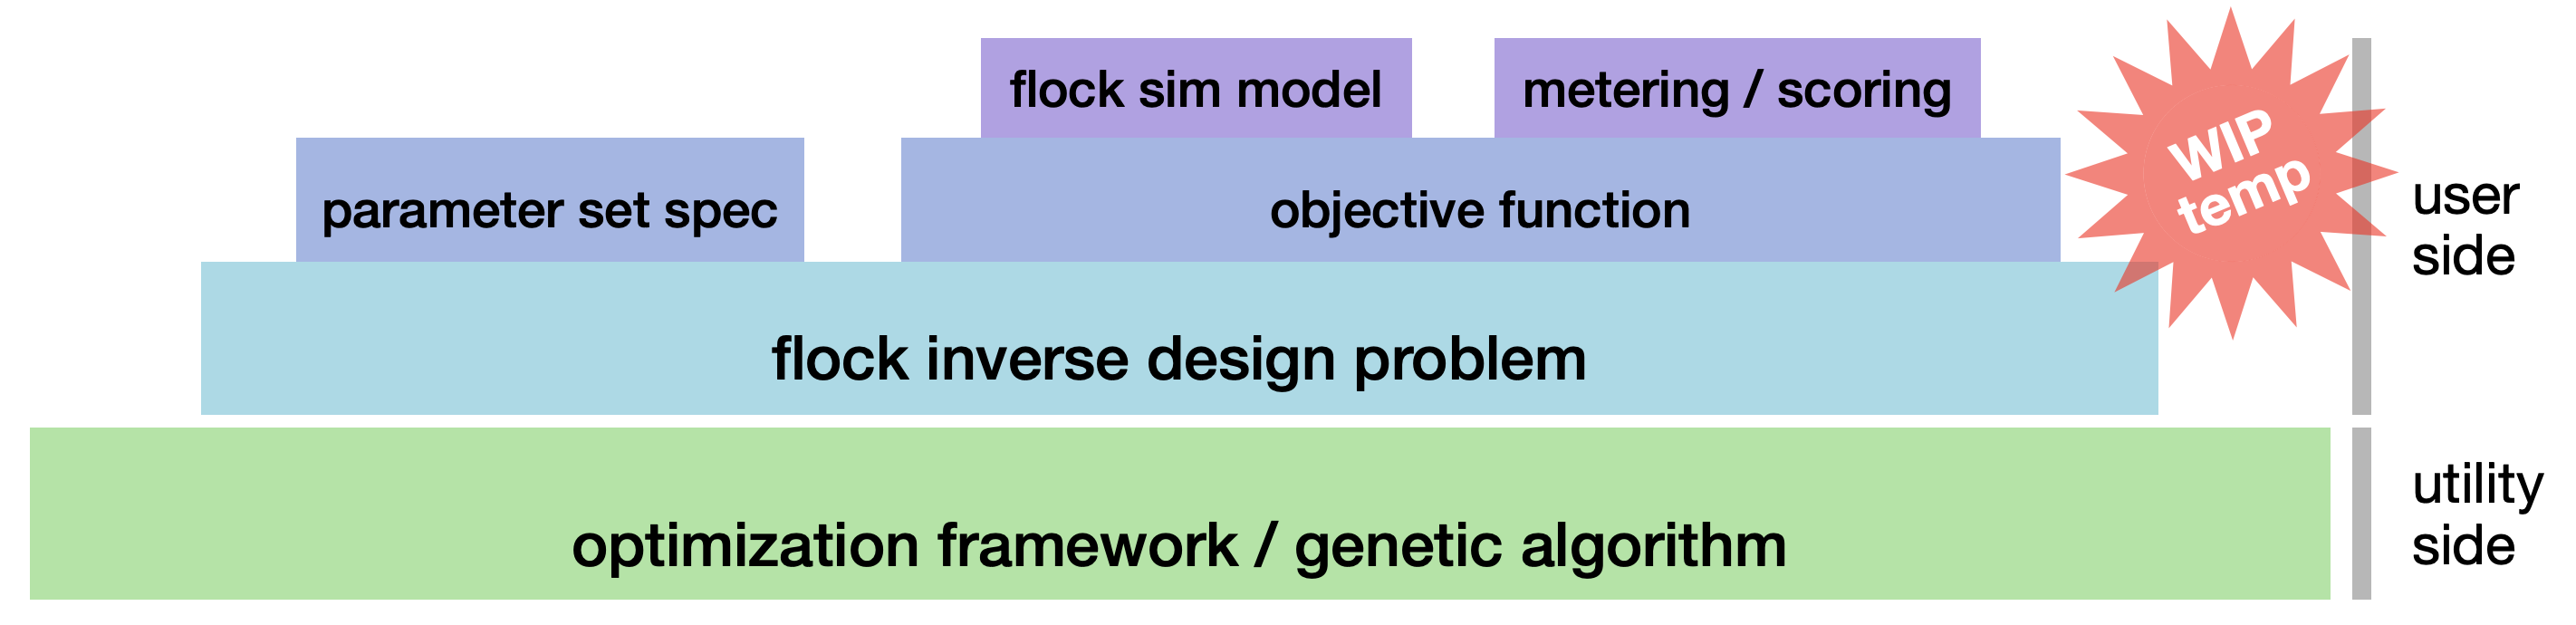
\includegraphics[width=0.9\linewidth]{images/temp_system_blocks.png}
    \caption{Overall structure of the flock optimization presented here. A generic optimization base (green) operates on a user's flock inverse design problem (blue). The user's description includes a parameter set specification and an objective function, the latter containing a flock simulator and score keeping utilities. [[[\textbf{TEMP}]]]}
    \label{fig:system_blocks}
\end{figure}

%%%%%%%%%%%%%%%%%%%%%%%%%%%%%%%%%%%%%%%%%%%%%%%%%%%%%%%%%%%%

\section{Related Work}
\label{sec:related}

Since the 1980s, many simulation-based models of bird flocks have been proposed. They have broadly similar intent, with many differences in their modeling philosophy and computational technique. These models include \textit{boids} and many others:
\citet{aoki_simulation_1982}, 
\citet{akira_okubo_dynamical_1986}, 
\citet{reynolds_flocks_1987},
\citet{heppner_stochastic_1990}, 
\citet{tu_artificial_1994},
\citet{vicsek_novel_1995},
\citet{toner_flocks_1998}, 
\citet{bajec_simulating_2005},
\citet{cucker_emergent_2007},
\citet{moskon_fuzzy_2007},
\citet{cavagna_seventh_2008},
\citet{bajec_organized_2009},
\citet{bhattacharya_collective_2010}
\citet{vasarhelyi_optimized_2018}
\citet{hoetzlein_flock2_2024}.

Early users of flock models found ``tuning'' their many parameters to be frustratingly difficult. This led to research on better tools for this task. This paragraph lists the works that most directly led to the technique described in this paper. An early, but not very successful, attempt at inverse design for flock simulations \citep{reynolds_evolved_1993} used \textit{genetic programming} \citep{koza_genetic_1992}. (GP is a variation on the \textit{genetic algorithm} (GA) \citep{holland_adaptation_1975}.) \citet{stonedahl_finding_2011} use a GA to search parameter spaces using an objective function running flock simulations based on NetLogo \citep{tisue_netlogo_2004}. Similarly \citet{demsar_evolution_2017} attempt ``to evolve collective behavior from scratch.'' \citet{vasarhelyi_optimized_2018} used a GA to tune flocking models suitable for the flight dynamics of a swarm of real drones. \citet{stolfi_escorting_2025} use evolutionary optimization to design robotic swarms for ``escorting'' tasks.

Most previous work on automatically tuning flock/multi-agent models has used \textit{reinforcement learning} (RL) \citep{sutton_reinforcement_1998} as the optimization technique. For example, recent excellent work in \citet{cornelisse_building_2025} and \citet{cusumano-towner_robust_2025} on high quality \textit{driver agents} for a multi-agent traffic simulation. They use \textit{self-play} where agents learn (``bootstrap'') from interacting with each other. The technique described in this paper also has an aspect of self-play as flockmates learn to synchronize with each other.

As this paper was being drafted, a preprint was posted \citep{brambati_learning_2025} using reinforcement learning with an objective function very similar to the one used here. 

Notable, if somewhat tangential: \citet{jaderberg_human-level_2019} uses a hybrid approach to learn human-level game-playing agents for multiplayer games. It uses population-based reinforcement learning, which combines aspects of RL, population-based GA, and the self-play mentioned above.

The approach used here was developed as part of a larger ongoing collaboration investigating new approaches to optimization of multi-agent motion. [[[\textbf{...My impulse here is to cite ``(Shang, 2025)'' Matthew's thesis. But I don't know where/how to do that, nor if it is appropriate. Suggestions appreciated...}]]]

\section{Description of the Technique}
\label{sec:Description}

This section discusses the various components of the optimization process for adjusting parameters of a flock, or other kinds of multi-agent motion model. See Figure \ref{fig:system_blocks} for a diagram.

\subsection{Optimization with Genetic Algorithms}
\label{subsec:Optimization_with_GA}

[[[\textbf{...make some mention of \textit{LazyPredator}...}]]]

Optimization can be used to find a set of simulation parameters that best fit the behavioral goals, as given by an objective function. The approach described here uses a \textit{genetic algorithm} (GA), a technique based loosely on concepts of biological evolution, as seen in the natural world. Genetic algorithms were first described by \citet{holland_adaptation_1975}. Evolution was first described by \citet{darwin_origin_1859}.

A genetic algorithm maintains a \textit{population} of candidate solutions. Usually, the population contains a fixed number (tens to thousands) of candidate solutions, often called \textit{individuals}. Typically, each individual is a fixed-sized vector of numeric parameter values. The population may be further divided into \textit{demes} or \textit{islands}, representing smaller breeding subpopulations. This is thought to promote diversity by pursuing different solutions in parallel. In an island model, there is usually some kind of \textit{migration} where individuals occasionally move from one island to another.

A GA is a population-based stochastic approach to optimization and discovery. Unlike random search, they proceed by a random process guided by the frequency of useful partial solutions in the population, a model of biological gene frequency in a species' \textit{genome}.

A GA's ``genome'' changes over time under the influence of the objective function. For example, a model parameter might be changed by \textit{mutation}: adding a signed zero-centered random value, offsetting the parameter by a small amount from its previous value. Perhaps more importantly individuals are modified by \textit{crossover} where two \textit{parent} individuals are recombined to create a new \textit{offspring}. In a rough model of biological crossover involving parental DNA, two parental parameter sets are merged into one, by taking each parameter at random from one parent or the other (called uniform crossover).

Many variations on genetic algorithms have been developed over the years. Sometimes, the entire population of individuals is updated in parallel, as a \textit{generation}, and that process is repeated tens to hundreds of times. The approach used here, known as \textit{steady state genetic algorithms} (SSGA) updates individuals one at a time \citep{syswerda_study_1991}. If a generational GA is run for $G$ generations with a population of $P$ individuals, a corresponding SSGA would be run for $G{\times}P$ steps. See Figure \ref{fig:temp_evo_update} for a diagram of the SSGA update cycle, along with the ``tournament of three individuals'' used in this work. A preexisting GA framework called \textit{LazyPredator} was used for this work.

[[[\textbf{...negative selection for diveristy preservation}]]]

\subsection{Objective Function}
\label{subsec:ObjectiveFunction}

This work is based on optimizing a set of parameters for a flock (multi-agent motion) model. Optimization procedures are guided by an \textit{objective function}. In many optimization problems, the overall objective is a combination of several, potentially contradictory goals, called multi-objective optimization. 

To motivate this concept, consider building a bridge over a river. A key goal is that the bridge is reliable: that it will carry the required loads without collapsing. Another important goal is to minimize the cost of building the bridge. These criteria are directly opposed. A very strong bridge is reliable but costly. A very cheap bridge is unlikely to be reliable. This trade-off is often called \textit{Pareto optimality}. Tuples of such Pareto optimal values form the \textit{Pareto front}, see Figure \ref{fig:MOF_HV}(b).

Other types of multi-objective optimization have less contradictory goals. The multi-agent motion problem seems to fall into this category. For this application, all that is required is to find parameter sets so that each of the objectives can be well satisfied, see Figure \ref{fig:MOF_HV}(c).

\subsection{Multi-Objective Optimization}
\label{subsec:Multi-Objective}

Early genetic algorithms were used for problems with a single scalar fitness value. These have the advantage of having a \textit{total order}. However, like the bridge example above, many problems inherently have \textit{multiple objectives} (see Figure \ref{fig:MOF_HV}(B)). The flock optimization problems addressed here seem to be in the ``mostly compatible'' type of multiple objective problems (see Figure \ref{fig:MOF_HV}(C)) so can be solved with \textit{scalarization}. A scalarizer maps from multiple objective values to a single scaler value that somehow summarizes the multiple objective values.

A simple and commonly used scalarizer is called \textit{hypervolume}, which simply multiples together the components of a multiple objective value. The name hypervolume refers to a \textit{n}-dimensional box whose edges correspond to the components of a multiple objective value. Hypervolume has the property that its value changes in proportion to changes in each component.

So for example, the hypervolume goes up (or down) if any component goes up (or down) --- as long as none of the components are zero, which ``hides'' contributions of other components. To avoid this, the hypervolume varient used here remaps the fitness range from [0, 1] to [$\epsilon$, 1] before taking the product. ($\epsilon$ is 0.01 for the ``normalized fitness'' values used here.)

%%%%%%%%%%%%%%%%%%%%%%%%%%%%%%%%%%%%%%%%%%%%%%%%%%%%%%%%%%%%

\begin{figure}[t]
    \centering
    % 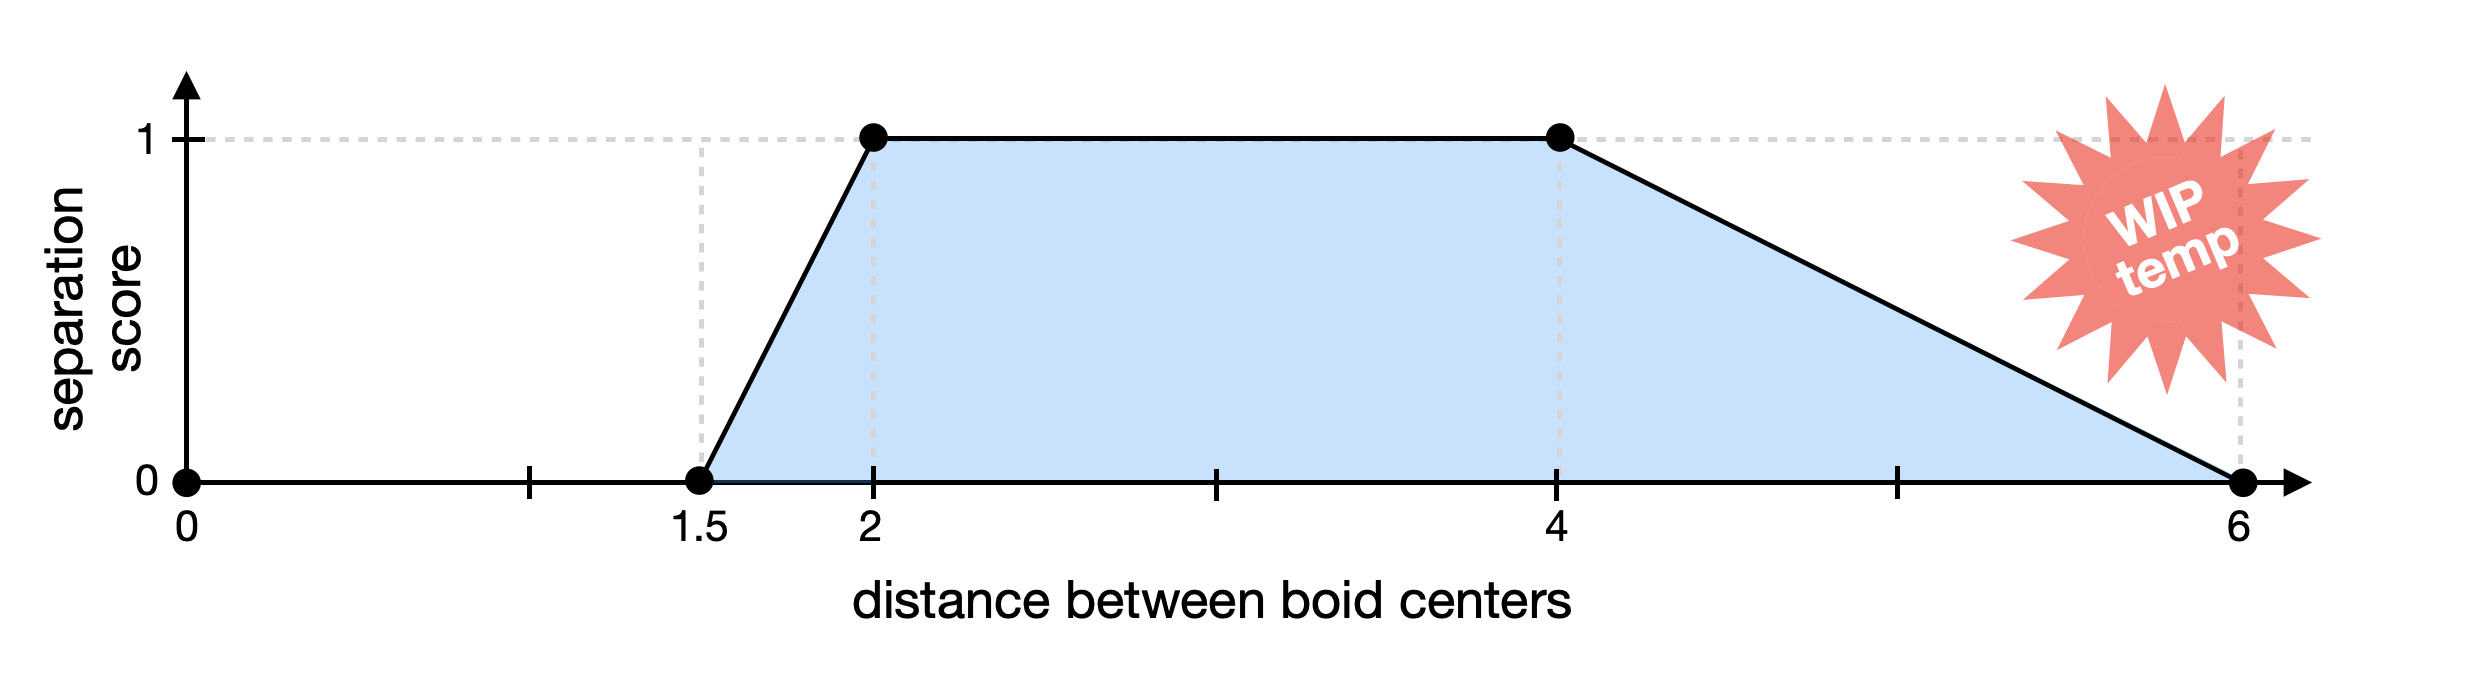
\includegraphics[width=0.9\textwidth]{images/temp_sep_score.png}
    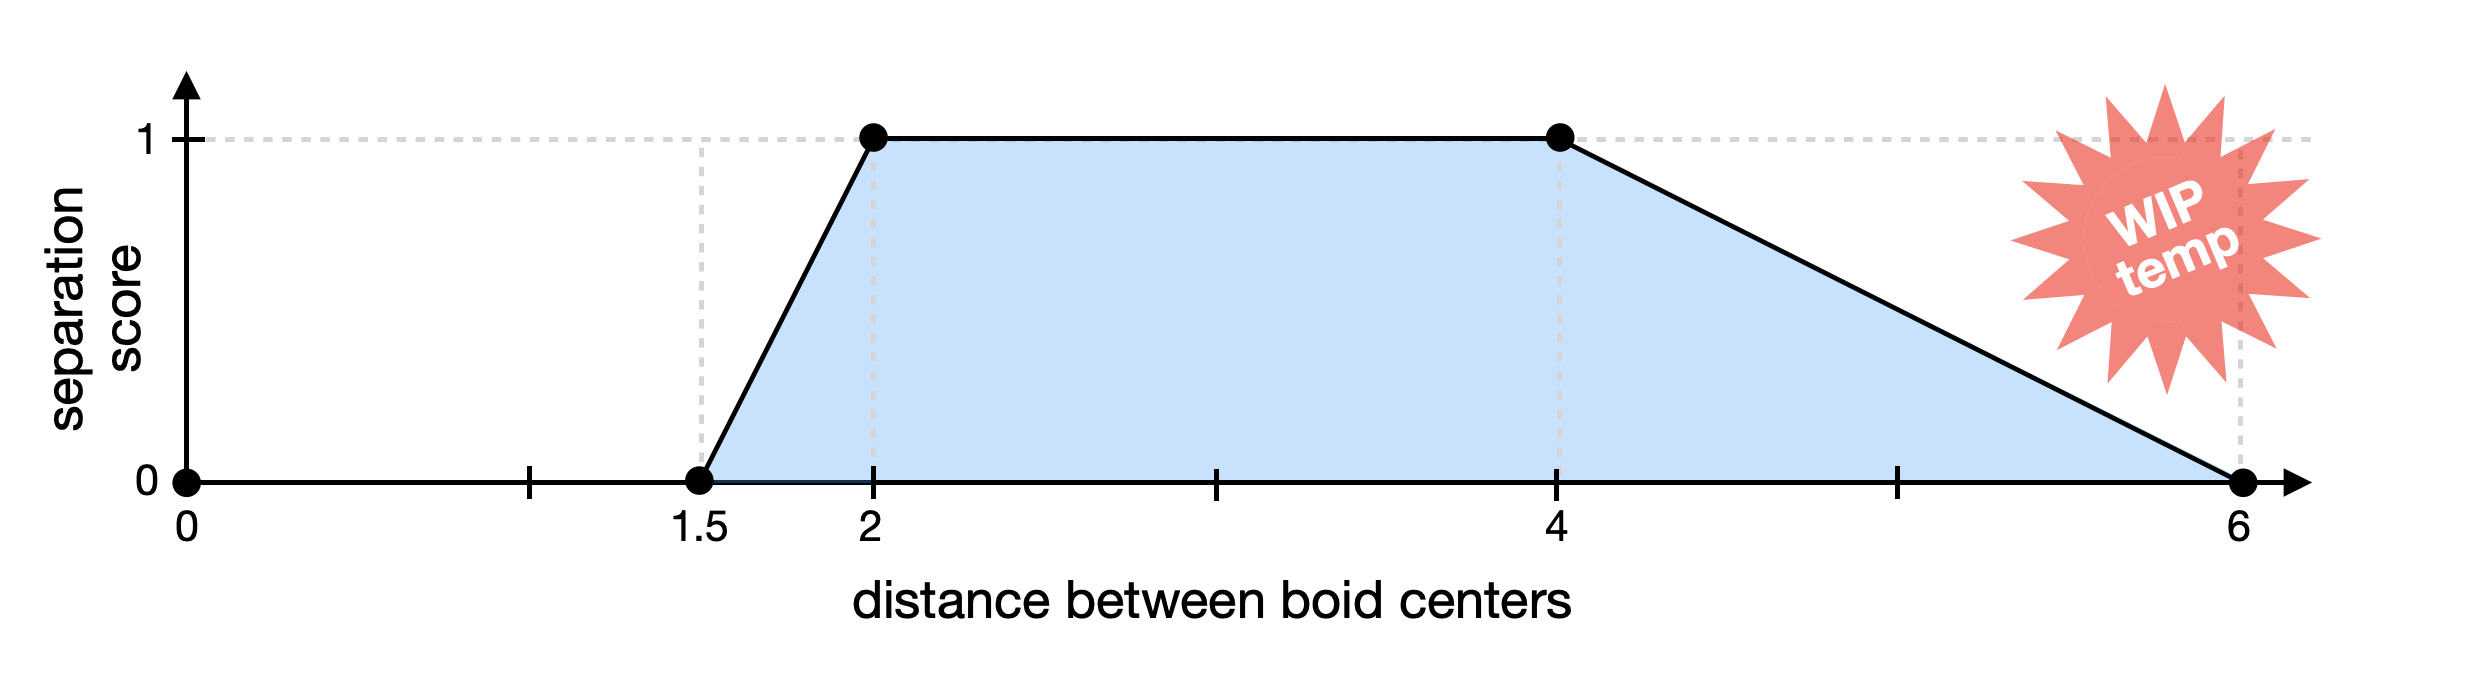
\includegraphics[width=0.9\linewidth]{images/temp_sep_score.png}
    \caption{Score for desired \textit{separation} distance to a boid's nearest neighbor. This function is highest when the centers of two boids are between 2 and 4 body diameters apart. The default boid body diameter is 1. The \textit{separation} score for an entire flock simulation is the average of this function, over all boids, on all simulation steps. [[[\textbf{...should I say ``all boid-steps''?...}]]]}
    \label{fig:SeparationScore}
\end{figure}
%%%%%%%%%%%%%%%%%%%%%%%%%%%%%%%%%%%%%%%%%%%%%%%%%%%%%%%%%%%%

%%%%%%%%%%%%%%%%%%%%%%%%%%%%%%%%%%%%%%%%%%%%%%%%%%%%%%%%%%%%

\begin{figure}[t]
    \centering
    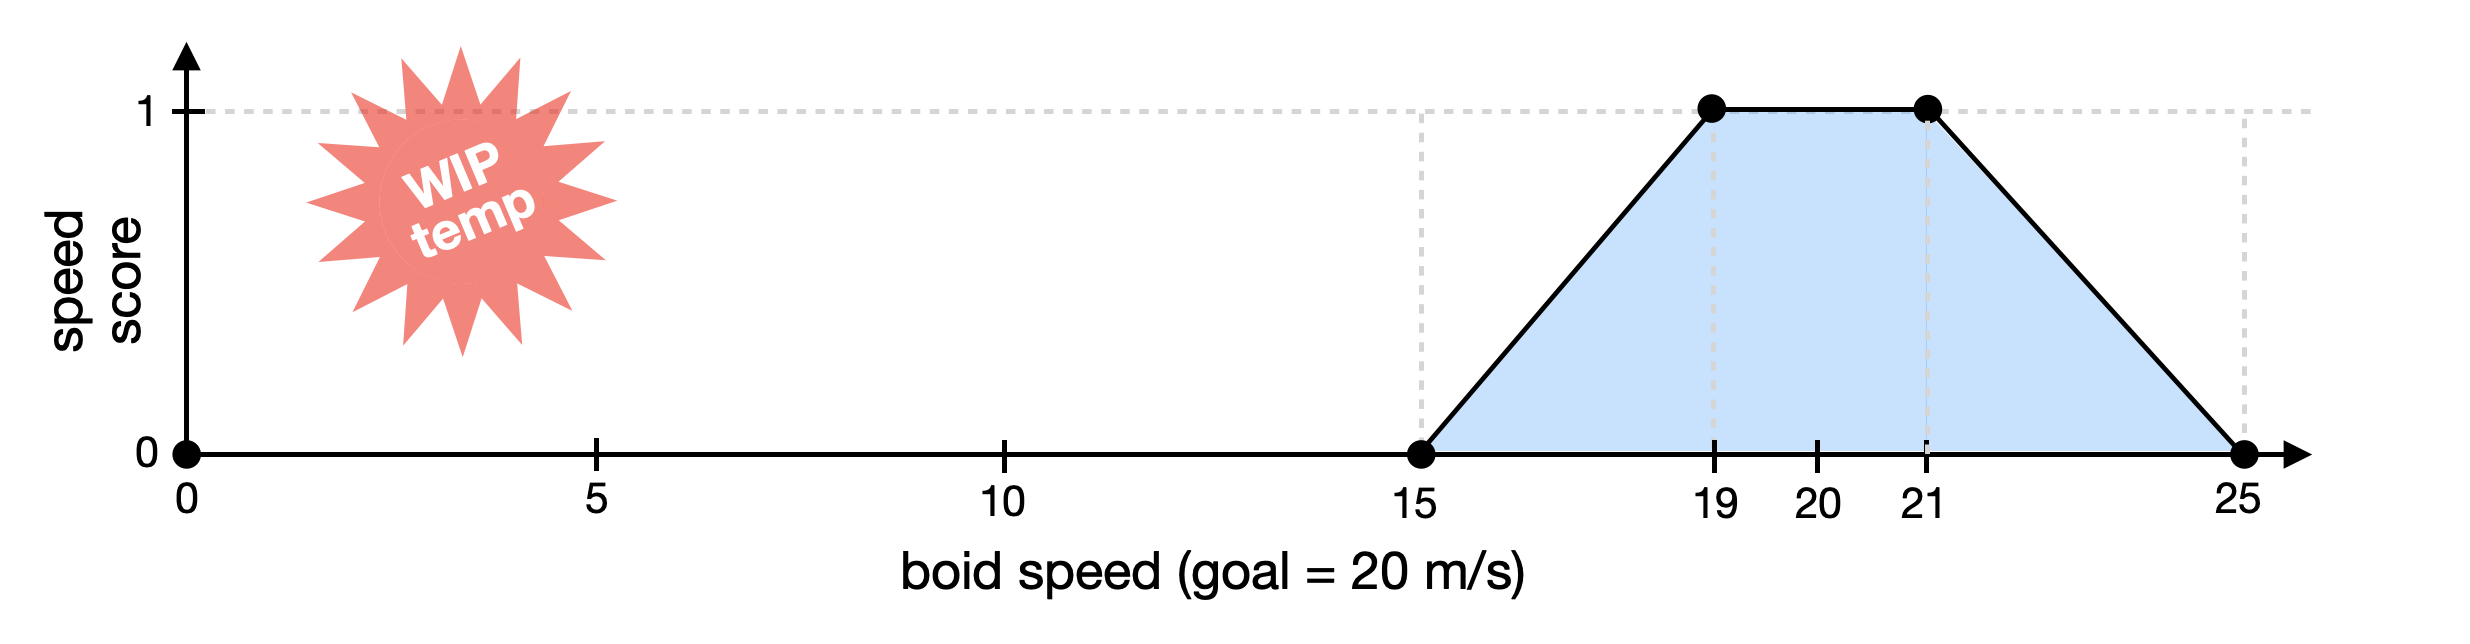
\includegraphics[width=0.9\linewidth]{images/temp_speed_score.png}
    \caption{Score for desired boid \textit{speed}, here $\sim$20 meters per second. This function is highest when speed is between 19 and 21 m/s and falls off to zero outside that range. The \textit{speed} score for an entire flock simulation is the average of this function, over all boids, on all simulation steps. [[[\textbf{boid-steps?}]]]}
    \label{fig:speed_score}
\end{figure}

%%%%%%%%%%%%%%%%%%%%%%%%%%%%%%%%%%%%%%%%%%%%%%%%%%%%%%%%%%%%

%%%%%%%%%%%%%%%%%%%%%%%%%%%%%%%%%%%%%%%%%%%%%%%%%%%%%%%%%%%%

\begin{figure}[t]
    \centering
    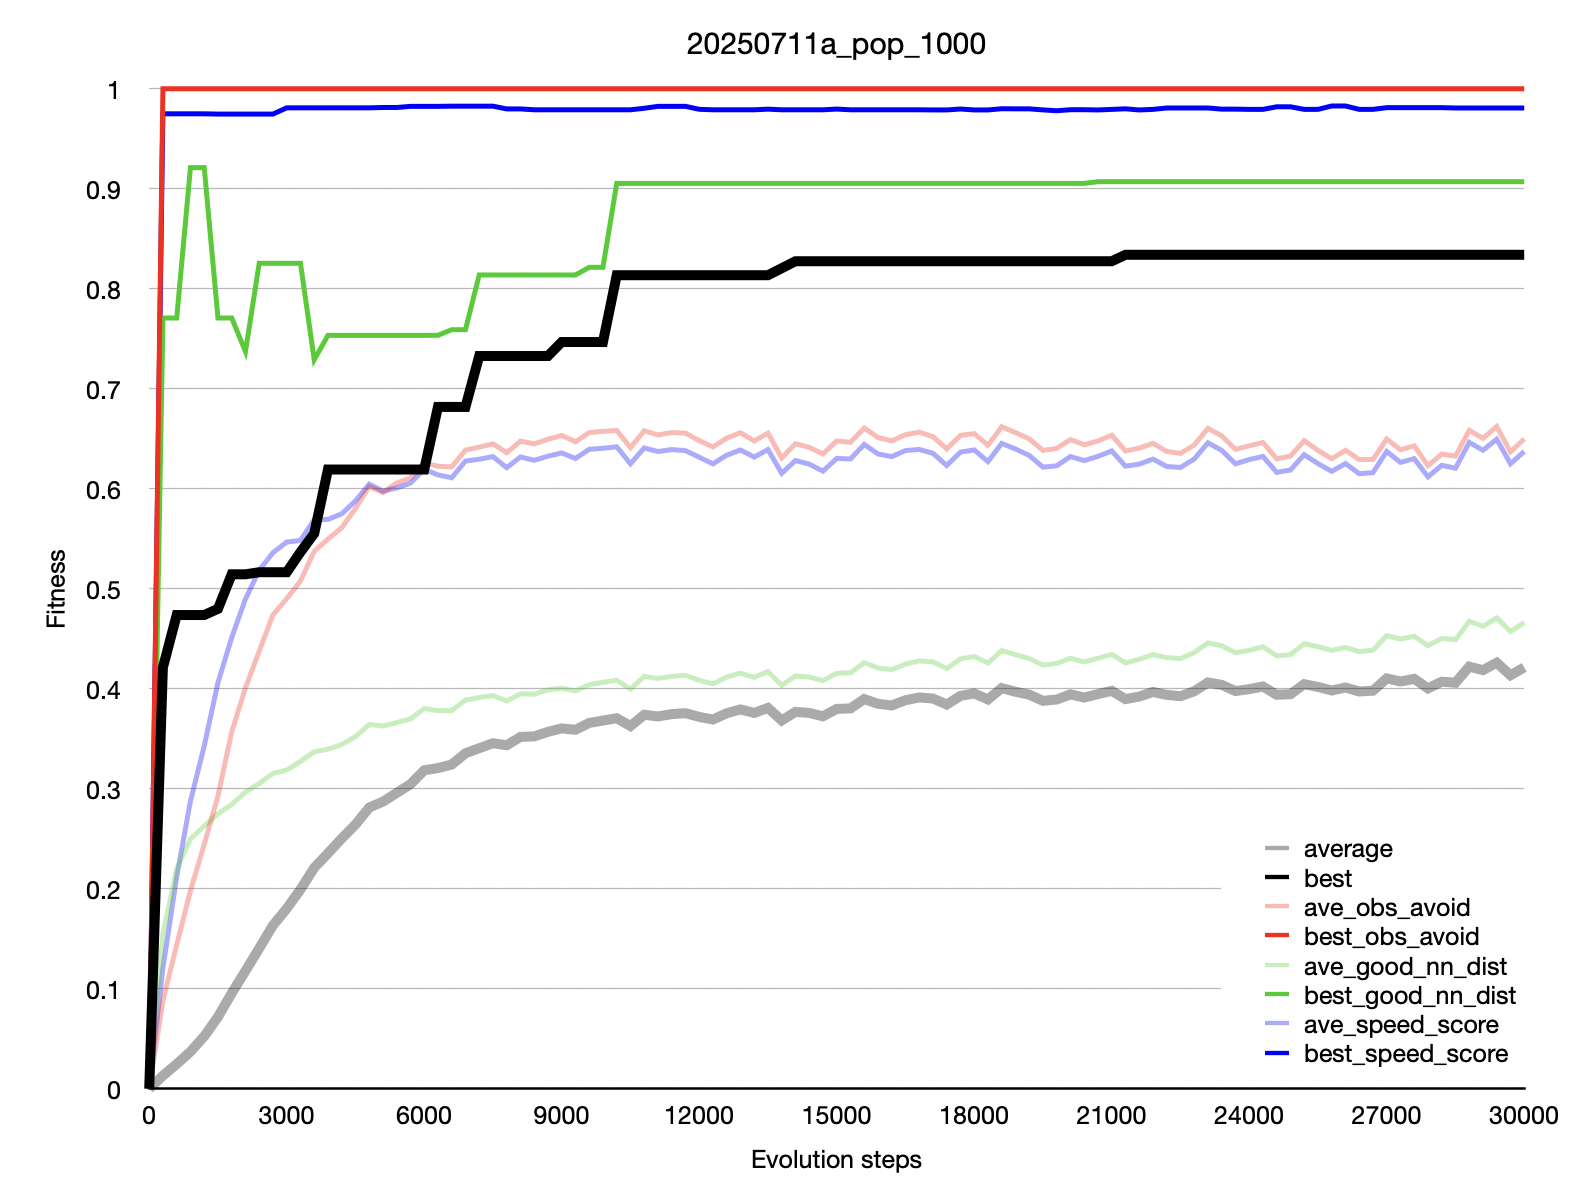
\includegraphics[width=\linewidth]{images/temp_fit_plot.png}
    \caption{Plot of scalarized fitness (and its component metrics) over 30,000 steps of evolutionary time. The black bold trace (ending at 0.83) is the cumulative best population fitness. The bold gray trace (bottommost) is population average fitness. The colored traces correspond to best and average values (saturated and pastel) for the three component fitness objectives: obstacle avoidance (red), separation (green), and speed (blue). Data from run 20250711a. [[[\textbf{TEMP}]]]}
    \label{fig:fit_plot}
\end{figure}
%%%%%%%%%%%%%%%%%%%%%%%%%%%%%%%%%%%%%%%%%%%%%%%%%%%%%%%%%%%%

\section{Parameter set for a flocking model}
\label{sec:parameter_set}

The focus of this paper is on the \textit{inverse design}, the optimization of parameter sets to achieve behavior under the direction of an objective function. As such, details of a particular flocking model are largely off-topic. However, just to ground the discussion for readers unfamiliar with flocking models, a quick overview is given here.

Most flock models are written from the perspective of an individual ``boid'' at a single time step. The boid identifies its neighbors. (The model used in this work uses \textit{topological distance} to find the seven nearest neighbors.) The boid reacts to its neighbors by computing \textit{steering forces} related to their distance and angle. It may also need to steer to avoid obstacles. These component steering forces are combined (often by 3D vector addition) then applied to the boid's physics model (often a simple \textit{self-propelled particle} model).

Each of these steering behaviors has parameters, such as weights, distances, and angles. (For example, what is the minimum amount of time before a predicted collision with an obstacle at which the boid should start steering to avoid?) There are also parameters related to it physical model, such as the maximum force it can apply.

The collection of all these make up the flock's \textit{parameter set} which is adjusted by optimization according the the objective function. See Table \ref{table:flock-parameters} for a list of the parameter set used in these experiments.



\section{An objective function for flocking}
\label{sec:FlockingObjective}

Having described the components of the optimization framework for this inverse design project (see \nameref{sec:Description}), this section focuses on the specific objective(/fitness/loss) function that was used in this work to optimize a multi-agent motion model for flocking.

The objectives described below are based on measurements made during the flock simulation process. That is, in addition to running the simulation, ``bookkeeping'' code is run while updating each individual boid step, after a flock update, and at the end of a simulation. Those metrics are stored in the flock instance and queried by the evolutionary optimization framework in which the flock simulation is run.

\subsection{Objective for Separation}
\label{subsec:separation_objective}

A key observation is that the birds in a flock are grouped closely together but nearly always avoid colliding with flockmates. These goals (close together, no collisions) can be seen as a requirement that the distance between simulated boids fall within a certain distance interval. Specifically, for a given boid, we determine its nearest neighbor and measure the distance between their centers. A score is computed on the basis of that distance. See Figure \ref{fig:SeparationScore}. It is zero if either the distance is too small (potential collision) or too large (failure to form a dense flock). Within an acceptable distance range, its value is one. Outside that desired range, piecewise linear ramps transition down to zero.

An equally iconic property of natural flocks is that birds are \textit{aligned}, flying on nearly parallel paths with their neighbors. An interesting result of this work is that this alignment appears to \textit{emerge} from the ``acceptable neighbor distance'' criteria. It was \textbf{not} necessary to have an explicit optimization objective for alignment. The optimization for proper separation appears to \textbf{cause} the alignment.

\subsection{Objective for Obstacle Avoidance}
\label{subsec:avoidance_objective}

The example application in this work can be described as ``flocking in the presence of obstacles'' as shown in Figure \ref{fig:boid_flock}. At each time step, part of each boid's simulation is predicting future obstacle collisions and applying steering force to avoid them. The same code detects obstacle avoidance failures. In simulation, this is a matter of a boid having incorrectly passed through the surface of the obstacle. A kinematic constraint is invoked to move the boid back to the correct side of the boundary. This failure is recorded in a collision counter on each boid. At the end of the flock simulation this is turned into a normalized score of the total number of all collisions over the total number of boid-steps. (Typically in these experiments, a fitness test runs 200 boids for 500 simulation steps, so the final score is total number of collisions over 100,000.) 

For collision avoidance, the goal is not merely to \textit{reduce} the number of collisions but to effectively eliminate them. (An informal goal in these experiments has been {$\leq$}10 collisions per 100,000 boid-steps.) To express this, the normalized obstacle avoidance score (on [0, 1]) is exponentiated to the 500\textsuperscript{th} power. This pushes nearly the whole score's range down near zero, except for a small region near a perfect score of one. This effectively rejects flock parameter sets with more than a handful of collisions per flock simulation.

\subsection{Objective for Flight Speed}
\label{subsec:speed_objective}

Originally, following early boid models \citep{reynolds_flocks_1987}, each boid's flight speed was kinematically clipped to remain below 20 meters per second. Later, a third flock optimization objective was added to establish a target speed range. A new behavior was added to each boid to apply a force along its direction of motion to adjust its flight speed toward the desired range. The strength of this behavior became one of the flock parameters being optimized in the inverse flock design process.

Flight speed \textit{can} be left to “float” during optimization. Unfortuately there is an annoyingly large basin of attractions around not moving (speed=0). In any case, any given inverse design problem would likely imply a range of valid speeds. This suggests that the speed range should be given in the inverse design problem statement. For example, modeling a flock of finches and a flock of swallows would imply very different speed ranges. Figure \ref{fig:speed_score} shows a speed score function used in these experiments. It has a target range in the interval [19, 21] with a fixed support ramping down to zero outside that range.

\subsection{Adding an objective}
\label{subsec:add_objective}

[[[\textbf{...Make experiment with adding a goal for increasing path curvature. If it works describe here. Otherwise put it in \nameref{sec:future}...}]]]

%%%%%%%%%%%%%%%%%%%%%%%%%%%%%%%%%%%%%%%%%%%%%%%%%%%%%%%%%%%%

\begin{table}[t]
\centering
\begin{tabular}{ | l | c | c | }
    \hline
    % \multicolumn{3}{|c|}{Project Parameters} \\
    \textbf{Description} & \textbf{Value} & \textbf{Notes} \\
    \hline
    boids per flock & 200 &  \\
    flock simulation steps & 500 & $\sim$16.6 sec \\
    simulation time step & 1/30 seconds & \\
    \hline
    boid body diameter & 1 meter & \\
    boid body mass & 1 kilogram & \\
    boid max force & < 100 newtons & \\
    boid speed range & 19 to 21 m/s & \\
    obs avoid exponent & 500 & \\
    k nearest neighbors & 7 & cf. StarFlag \\
    \hline
    evolution population & 300 & individuals \\
    evolution steps & 30,000 &  SSGA steps \\
    equivalent generations & 100 & \\
    hypervolume epsilon & 0.01 & $\epsilon$ \\
    \hline
    run time: flock sim & $\sim$0.25 seconds & $200{\times}500$ \\
    run time: evolution & $\sim$2 hours & \\
    \hline
\end{tabular}
\caption{Detailed (``hyper'')parameters for the evolutionary inverse design framework. Run times are on a 2021 Apple Macbook Pro M1 Max.}
\label{table:HyperParameters}
\end{table}

\begin{table}[t]
\centering
\begin{tabular}{ | l | c | c | }
    \hline
    \textbf{Description} & \textbf{Range} & \textbf{Units} \\
    \hline
    max force & [0, 100] & newtons \\
    % min speed & [20, 20] & \textit{unused} \\
    % speed & [20, 20] & \textit{unused} \\
    % max speed & [20, 20] & \textit{unused} \\
    forward weight & [0, 100] & \textit{none} \\
    separate weight & [0, 100] & \textit{none} \\
    align weight & [0, 100] & \textit{none} \\
    cohere weight & [0, 100] & \textit{none} \\
    predictive avoid weight & [0, 100] & \textit{none} \\
    static avoid weight & [0, 100] & \textit{none} \\
    max dist separate & [0, 100] & meters \\
    max dist align & [0, 100] & meters \\
    max dist cohere & [0, 100] & meters \\
    angle separate & [-1, +1] & cos(a) \\
    angle align & [-1, +1] & cos(a) \\
    angle cohere & [-1, +1] & cos(a) \\
    fly away max dist & [0, 100] & meters \\
    min time to collide & [0, 10] & seconds \\
    \hline
\end{tabular}
\caption{Flock model parameters subject to optimization. These are a vector of scalar values, each with an associated range. They are initially randomized then optimized over time according to the objective function. [[[\textbf{...TEMP --- this is just a placeholder --- before paper submission I hope to make changes to this parameterization of the black box model, such as: removing the now unused min/max/speeds, moving from ``max distance'' parameters to exponents (and scales?) controlling falloff for the 7 nearest neighbors --- say something about the non-optimized ``Shared const/input parameters'' of FlockParameters ...}]]] }
\label{table:flock-parameters}
\end{table}

%%%%%%%%%%%%%%%%%%%%%%%%%%%%%%%%%%%%%%%%%%%%%%%%%%%%%%%%%%%%

\section{Conclusions}
\label{sec:Conclusions}

This work suggests that evolutionary optimization, via a genetic algorithm, can successfully optimize a set of parameters for a ``black box'' boid flocking model. This suggests that other similar multi-agent motion models --- for example, multi robot terrain search --- might well be solved using a genetic algorithm in a similar way, using an objective with some similarity to the one discussed in section \nameref{sec:FlockingObjective}.

[[[\textbf{should this be in the introduction? Say something about using deep reinforcement learning for flocks, etc.}]]] One advantage of using evolutionary optimization for this type of inverse design problem is that the multi-agent simulation can be treated as a ``black box.'' As such, there are few constraints on how the simulation is implemented. For example, to use \textit{stochastic gradient descent} (SGD) \citep{robbins_stochastic_1951} the flock model must be differentiable, either analytically or with \textit{automatic differentiation} \citep{baydin_automatic_2018}. Conversely, evolutionary optimization only requires the measured scalar fitness of a simulation, no gradients are used.

[[[\textbf{...I said this above, should it be here, or simply call back to it? \textit{An equally iconic property of natural flocks is that birds are aligned, flying on nearly parallel paths with their neighbors. An interesting result of this work is that this alignment appears to \textit{emerge} from the ``acceptable neighbor distance'' criteria. It was \textbf{not} necessary to have an explicit optimization objective for alignment...}}]]]

[[[\textbf{...say something about how increasing the evo pop size gives some advantage in being able to track more potential solutions, but that for a given number of evo steps, there are fewer ``updates per individual'' which reduces quality of optimization --- ``less parallel population, more sequential evolution''...}]]]

[[[\textbf{...similarly: for a long time I was using pop=500/steps=30000. Then I tried increasing pop, eventually to 1000. I was getting worse results. Today (20250724) I tried running for steps=60000, which did well reaching EOR best fitness of 88\% --- and separately with pop=150, which did poorly (72\%)...}]]]

\section{Limitations}
\label{sec:limitations}

[[[\textbf{...point of that that every run is a winner, often the objective is not well met --- fitness nearer 70\% than 80\% --- and the performance noticeably diminished --- happens maybe once in every 2 or 3 runs...}]]]

[[[\textbf{...for speed score and separation score: does it matter if the ramps on either side of the sweet spot are there? Should try a test...}]]]

[[[\textbf{...discuss the ``ignoring noise'' paper \citep{antipov_evolutionary_2025}...}]]]

\section{Future Work}
\label{sec:future}

[[[\textbf{...I plan to try adding a fourth objective --- perhaps for path curvature --- as an exercise to talk about more advanced inverse design problems --- but if not, it should be mentioned here...}]]]

[[[\textbf{...experiment with open space flocking --- no obstacles --- perhaps in conjunction with path curvature objective...}]]]

[[[\textbf{...perhaps try non-uniform \citep{montanari_optimal_2025} and non-reciprocal \citep{choi_flocking_2025} multi-agent models...}]]]

[[[\textbf{...mention a GP (rather than GA) version of this approach...}]]]

[[[\textbf{...say something about how I used three objectives to evolve flocking of the type shown in Fig. 1 --- maybe try an experiment with ``open air flocking'' to see if it will work with just separation score... --- ...so I did try this and the results were pretty boring, maybe it would look better after i add a fourth objective for path curvature...}]]]

\section{Acknowledgements}
\label{sec:ack}

This work is part of a larger project. Many thanks for conversations and camaraderie to my collaborators: Gilbert Bernstein, Matthew Shang, and Jennifer Luo. I also want to thank my long time ($\sim$30 year) friend and ALife colleague, Inman Harvey, whose deep insights taught me much about evolutionary computation and scholarship. Thanks to my family for loving support. [[[\textbf{revisit this}]]]
% Wahrman(?)
% flocking friends?

\bibliographystyle{apalike}
\bibliography{EvoFlock.bib}

%%%%%%%%%%%%%%%%%%%%%%%%%%%%%%%%%%%%%%%%%%%%%%%%%%%%%%%%%%%%

% Appendix / Supplemental Materials

% \appendix
% \onecolumn
% \section{Appendix}
% \label{sec:appendix}

\end{document}